
\section{Training Curves}\label{sec:graphs:training_curves}

Training curves plots the evaluation metric, or error estimation, with respect to epochs, the number of iterations in an iterative algorithm.

\subsection{katz-eig}

\FloatBarrier

\begin{figure}[h!]
  \centering
    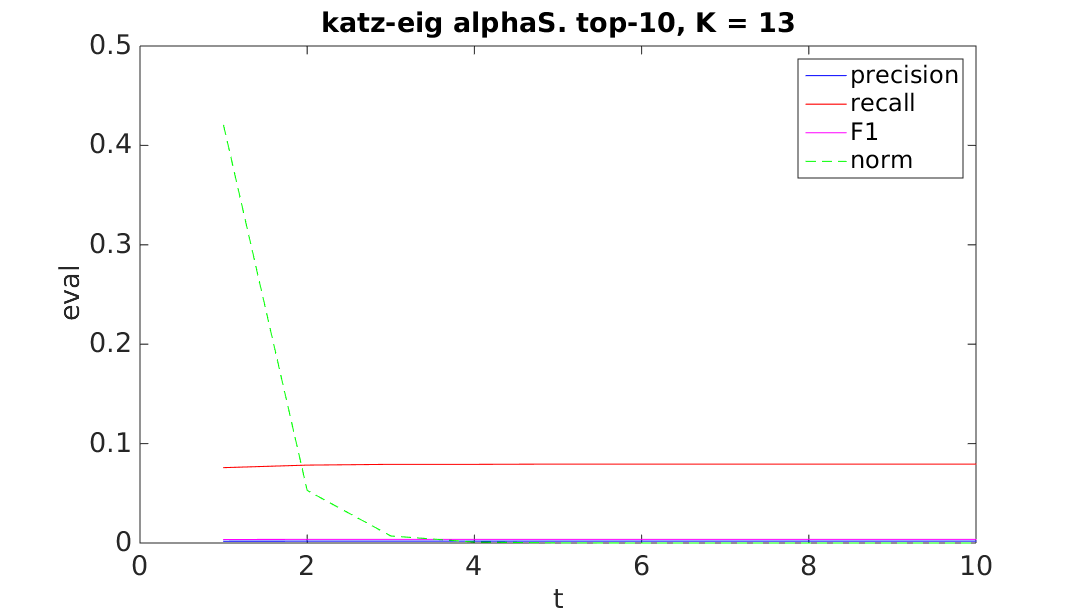
\includegraphics[width=0.8\textwidth]{fig/katzeig_t/alphaS_katzeig_t.png}
    \caption{\textit{alphaS}}
\end{figure}

\begin{figure}[h!]
  \centering
    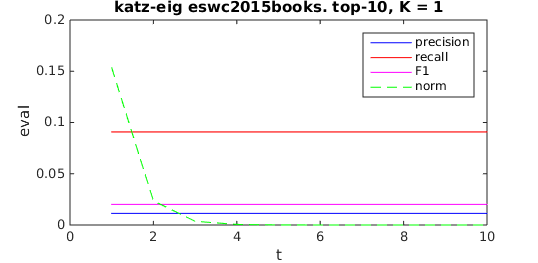
\includegraphics[width=0.8\textwidth]{fig/katzeig_t/eswc2015books_katzeig_t.png}
    \caption{\textit{eswc2015books}}
\end{figure}

\begin{figure}[h!]
  \centering
    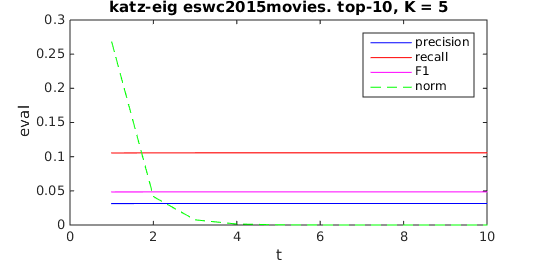
\includegraphics[width=0.8\textwidth]{fig/katzeig_t/eswc2015movies_katzeig_t.png}
    \caption{\textit{eswc2015movies}}
\end{figure}

\begin{figure}[h!]
  \centering
    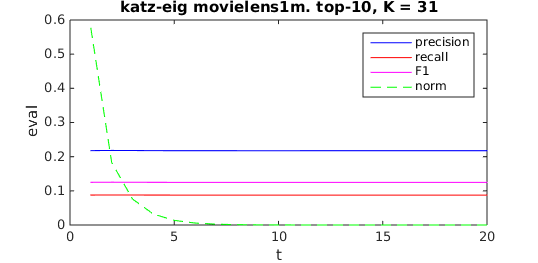
\includegraphics[width=0.8\textwidth]{fig/katzeig_t/movielens_katzeig_t.png}
    \caption{\textit{movielens1m}}
\end{figure}

\begin{figure}[h!]
  \centering
    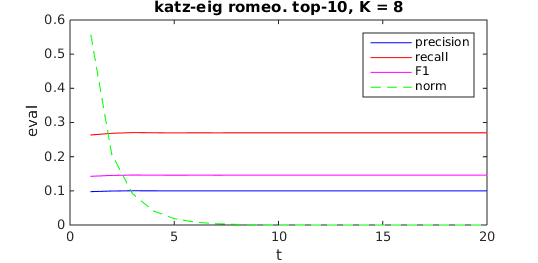
\includegraphics[width=0.8\textwidth]{fig/katzeig_t/romeo_katzeig_t.png}
    \caption{\textit{romeo}}
\end{figure}

\FloatBarrier


\subsection{link-analysis}

\begin{itemize}
    \item alpha
    \item alpha2
    \item eswc2015movies
    \item eswc2015music
    \item eswc2015books
    \item movielens1m
    \item romeo
\end{itemize}


